\begin{itemize}
We provide an elaborate analysis of the planned protest model as follows:
\item{Perfomance over the months}
    Fig.~\ref{fig:monthlyqs} provides the evaluation results of the model over the months with a breakdown of its sources. The QS reported is the weighted average of QS of all 10 countries.
    Twitter has a higher QS as multiple re-tweets of mention of future events in twitter is a direct indicator of the popularity of the event, the intent of people to join an event. While mention of Future events in News is simply a reporting of the event not much can be understood about the popularity of the event or about the people's support for the event. At the same time, twitter provides very little in terms of recall.
RSS has an average precision of 0.66 and a maximum recall 0.30 while
Twitter has an average precision of 0.81 while a max recall of 0.1.

\item{Country-wise perfomance}
    Table~\ref{tb:sourcewisecomparison} presents the perfomance of the planned protest model (for March 2014) for each of the 10 countries of interest. It also presents a source wise breakdown of perfomance. 
\end{itemize}









\begin{enumerate}

\item How Planned Protest model fared over the months?
Evaluation of Planned Protest Over the months

\item Contribution of Different Data Sources?
Evaluation of Each Individual Data Source,
    \begin{table*}[tb!]
        \small
        \centering
        \caption{\label{tb:sourcewisecomparison} Comparing forecasting accuracy of
        RSS vs Twitter}
        \begin{tabular}{|*{7}{c|}}
            \hline
            & \multicolumn{3}{ |c| }{News/Blogs} & \multicolumn{3}{ |c| }{Twitter}\\
            \hline
            Country & QS & Precision & Recall & QS & Precision & Recall\\
            \hline
            AR &3.14&0.32&0.69&3.52&0.78&0.14\\
            BR &3.14&0.48&0.54&0.00&0.00&0.00\\
            CL &3.06&0.91&0.67&3.52&1.00&0.23\\
            CO &2.74&0.90&0.56&3.30&1.00&0.15\\
            EC &0.00&0.00&0.00&2.32&1.00&0.06\\
            MX &2.96&0.88&0.25&3.14&1.00&0.02\\
            SV &3.22&1.00&0.03&0.00&0.00&0.00\\
            PY &3.38&1.00&0.16&3.84&1.00&0.04\\
            UY &3.24&1.00&0.29&0.00&0.00&0.00\\
            VE &3.80&1.00&0.36&3.68&0.97&0.33\\
            ALL &3.34&0.69&0.35&3.62&0.97&0.15\\
            \hline
        \end{tabular}
    \end{table*}

\item Brazilian June Protests and Venezuelan February Protests 
   
\item Different Evaluation criteria
   1. Varying Time Constraint from 7 to 1

\end{enumerate}




\begin{figure}
    \includegraphics[width=0.5\textwidth]{venezuela}
    \caption{Venezuelan Protests}
\end{figure}

\begin{figure}
    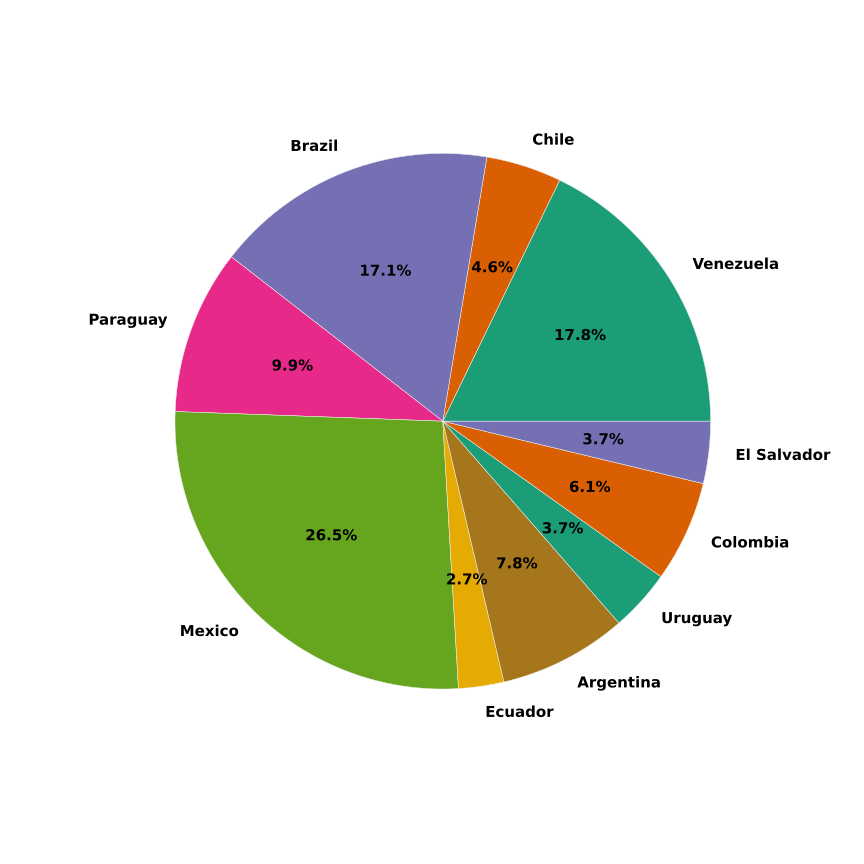
\includegraphics[width=0.5\textwidth]{gsr_distribution}
    \caption{GSR Distribution From 2012-11 to 2014-03}
\end{figure}


\begin{figure}
    \includegraphics[width=0.5\textwidth]{venezuela_violent}
    \caption{Venezuelan Violent Protests}
\end{figure}


\begin{figure}
    \includegraphics[width=0.5\textwidth]{brazil_june}
    \caption{Brazil June Protests}
\end{figure}

\begin{figure}
    \includegraphics[width=0.5\textwidth]{eventDateVsDate_brazil}
    \caption{Date of Prediction vs Forecasted Date Brazil}
\end{figure}

\begin{figure}
    \includegraphics[width=0.5\textwidth]{eventDateVsDate_venezuela}
    \caption{Date of Prediction vs Forecasted Date Venezuela}
\end{figure}

\begin{figure}
    \includegraphics[width=0.5\textwidth]{monthlyqs.pdf}
    \caption{Date of Prediction vs Forecasted Date Venezuela}
\end{figure}





%\begin{figure}
%    \centering
%    \begin{subfigure}[b][0.3\textwidth]
%        \includegraphics[width=\textwidth]{venezuela.png}
%        \caption{Venezuelan Protests}
%        \label{fig:Venezuela_feb}
%    \end{subfigure}
%    \begin{subfigure}[b][0.3\textwidth]
%        \includegraphics[width=\textwidth]{brazil_june.png}
%        \caption{Brazilian Riots in June}
%        \label{fig:Brazil_june}
%    \end{subfigure}
%\end{figure}
